% graph articulation point
% https://www.geeksforgeeks.org/articulation-points-or-cut-vertices-in-a-graph/
% https://www.hackerearth.com/practice/algorithms/graphs/articulation-points-and-bridges/tutorial/
% http://www.cs.kent.edu/~aleitert/iga/slides/04ArtPointsBridges.pdf
% https://iq.opengenus.org/find-articulation-points-or-cut-vertices-in-a-graph/
% Introduction to Algorithms 3rd Edition - Page 621

% http://www.cs.kent.edu/~aleitert/iga/slides/04ArtPointsBridges.pdf
\section{Puntos de articulación}\label{articulation-points}
Un vértice \( v \) es un punto de articulación (o vértice de corte), si al eliminar el vértice \( v \) del grafo aumenta el número de componentes conectados. Es decir, genera algunos vértices inalcanzables para otros, se desconecta el grafo.

\begin{figure}[H]
	\centering
	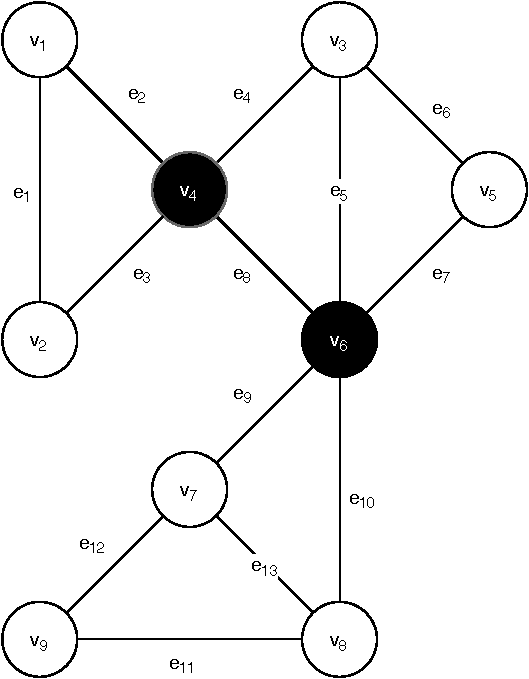
\includegraphics[width=0.4\linewidth]{document/ArticulationPoints/images/example-of-articulation-points}
	\caption{Ejemplo de grafo con dos puntos de articulación \( v_4 \) y \( v_6 \).}
	\label{fig:connected-disconnected-graph}
\end{figure}